%!TEX root = ../systemnahe-programmierung.tex

\chapter{Implementierung}\label{implementierung}

\begin{figure}[htbp]
\centering
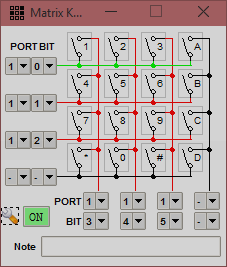
\includegraphics{images/keypad-screenshot}
\caption{Konfiguration des Nummernfeldes}
\end{figure}

Für die Simulation des Nummernfeldes wird das \emph{Matrix Keypad} der
\emph{MCU 8051 IDE} verwendet. Als Erstes muss die Pin-Belegung
konfiguriert werden. Im Bild kann man sehen, dass das Nummerfeld auf
Port 1 erreichbar ist. Diese Einstellung kann auch in die IDE import
werden (siehe Anhang).

\begin{Shaded}
\begin{Highlighting}[]
\NormalTok{keypad      }\DataTypeTok{equ} \NormalTok{P1              }\CommentTok{;Matrix keypad}
\NormalTok{col1        }\DataTypeTok{equ} \NormalTok{keypad}\FloatTok{.3}        \CommentTok{;Column 1}
\NormalTok{col2        }\DataTypeTok{equ} \NormalTok{keypad}\FloatTok{.4}        \CommentTok{;Column 2}
\NormalTok{col3        }\DataTypeTok{equ} \NormalTok{keypad}\FloatTok{.5}        \CommentTok{;Column 3}

\NormalTok{value       }\DataTypeTok{equ} \NormalTok{30H             }\CommentTok{;Value of pressed button}
\NormalTok{pressed     bit 00H             }\CommentTok{;Was the button just pressed?}
\NormalTok{secure_mode bit}\BaseNTok{ 01h             }\CommentTok{;Is the user logiged in?}
\end{Highlighting}
\end{Shaded}

Zusätzlich zu den Bits für das Nummernfeld werden auch noch drei
Variablen definiert:

\begin{itemize}
\itemsep1pt\parskip0pt\parsep0pt
\item
  \texttt{value}: Wert der gedrückten Taste
\item
  \texttt{pressed}: Ob schon eine Taste gedrückt wurde (wird
  zurückgesetzt, wenn auf ein neuen Tastendruck gewartet wird)
\item
  \texttt{secure\_mode}: In welchem Zustand die Alarmsicherung ist (0
  für ausgeschaltet, 1 für eingeschaltet)
\end{itemize}

\begin{Shaded}
\begin{Highlighting}[]
\FunctionTok{get_button:}
    \NormalTok{clr pressed}

    \CommentTok{;Check first row}
    \KeywordTok{mov} \NormalTok{value,#}\DecValTok{1}                \CommentTok{;Start value is first number on row}
    \KeywordTok{mov} \NormalTok{keypad, #11111110B      }\CommentTok{;Mark first row}
    \NormalTok{acall check_col1            }\CommentTok{;Check all columns }

    \CommentTok{;If button was pressed in row, jump out of function}
    \KeywordTok{jb} \NormalTok{pressed, found_button    }
 
    \KeywordTok{mov} \NormalTok{value,#}\DecValTok{4}
    \KeywordTok{mov} \NormalTok{keypad, #11111101B}
    \NormalTok{acall check_col1}
 
    \KeywordTok{jb} \NormalTok{pressed, found_button}
 
    \KeywordTok{mov} \NormalTok{value,#}\DecValTok{7}
    \KeywordTok{mov} \NormalTok{keypad, #11111011B}
    \NormalTok{acall check_col1}
 
    \KeywordTok{jb} \NormalTok{pressed, found_button}

    \KeywordTok{jmp} \NormalTok{get_button}
\end{Highlighting}
\end{Shaded}

Die Zeilen des Nummernfeldes werden nacheinander überprüft. Dabei wird
zuerst \texttt{value} auf den Wert der ersten Taste aus der Reihe
gesetzt. Danach werden alle Reihen außer die ausgewählte auf \texttt{1}
gesetzt und zur Funktion \texttt{check\_col1} gesprungen, die die
Spaltenüberprüfung für die ausgewählte Reihe startet. Nach jeder Reihe
wird überprüft, ob schon eine Taste gedrückt wird. Ist dies der Fall,
dann wird aus der Funktion gesprungen. Wenn alle Reihen überprüft wurden
und kein Tastendruck erkannt wurde, wird die Überprüfung wieder von vorne
begonnen.

\begin{Shaded}
\begin{Highlighting}[]
\FunctionTok{check_col1:}
    \CommentTok{;If button wasn't pressed, jump to next colum}
    \KeywordTok{jb} \NormalTok{col1, check_col2}

    \CommentTok{;If button was pressed, wait for end of button press}
    \KeywordTok{jnb} \NormalTok{col1,}\DecValTok{$}

    \CommentTok{;Set bit that key was pressed}
    \KeywordTok{setb} \NormalTok{pressed}
    \KeywordTok{ret}
\end{Highlighting}
\end{Shaded}

Wenn in der ersten Spalte kein Tastendruck entdeckt worden ist, wird zu
\texttt{check\_col2} gesprungen, die die nächste Spalte überprüft.
Sollte die Taste aber gedrückt sein, dass muss erst auf das Ende des
Tastendrucks gewartet werden. Dafür wird einfach zur gleichen Zeile der
Überprüfung gesprungen. Dach wird noch das Bit für \texttt{pressed} auf
\texttt{1} gesetzt.

\begin{Shaded}
\begin{Highlighting}[]
\FunctionTok{check_col2:}
    \KeywordTok{jb} \NormalTok{col2, check_col3}
    \KeywordTok{jnb} \NormalTok{col2,}\DecValTok{$}
    \KeywordTok{inc} \NormalTok{value           }\CommentTok{;Increment the start value from row}
    \KeywordTok{setb} \NormalTok{pressed}
    \KeywordTok{ret}
\end{Highlighting}
\end{Shaded}

Die Überprüfung der nächsten Spalten funktioniert fast identisch. Der
einzige Unterschied findet bei einem erfolgreichem Tastendruck statt. Da
der Wert der Taste verschiedene Werte hat, muss der Inhalt von
\texttt{value} noch angepasst werden. Dafür wird einfach um den
Unterschied inkrementiert (in diesem Fall 1).

\begin{Shaded}
\begin{Highlighting}[]
\FunctionTok{check_pin:}
    \CommentTok{;Check first pin (4)}
    \NormalTok{acall get_button}
    \KeywordTok{mov} \NormalTok{A, value}
    \KeywordTok{cjne} \NormalTok{A, #}\DecValTok{4}\NormalTok{, check_pin}

    \CommentTok{;Check second pin (2)}
    \NormalTok{acall get_button}
    \KeywordTok{mov} \NormalTok{A, value}
    \KeywordTok{cjne} \NormalTok{A, #}\DecValTok{2}\NormalTok{, check_pin}

    \CommentTok{;Check third pin (6)}
    \NormalTok{acall get_button}
    \KeywordTok{mov} \NormalTok{A, value}
    \KeywordTok{cjne} \NormalTok{A, #}\DecValTok{6}\NormalTok{, check_pin}

    \CommentTok{;Check fourth pin (8)}
    \NormalTok{acall get_button}
    \KeywordTok{mov} \NormalTok{A, value}
    \KeywordTok{cjne} \NormalTok{A, #}\DecValTok{8}\NormalTok{, check_pin}

    \CommentTok{;Toggle secure mode of the system}
    \NormalTok{cpl secure_mode}
\end{Highlighting}
\end{Shaded}

Die Hauptfunktion ist \texttt{check\_pin}. Sie ruft viermal die
\texttt{get\_button}-Funktion auf und überprüft, ob der gelieferte
Tastendruck dem gewünschtem gleicht. Sollte dies einmal nicht der Fall
sein, dann wird die Suche von vorne angefangen. Aber wurde die
Ziffernfolge erfolgreich eingegeben, dann wird der Alarm-Modus
gewechselt. Die Zifferfolge lässt sich sehr leicht ändern, unter anderem
auch in der Länge.
